%MARCOS RIAL DOCAMPO
%Parte del documento principal TFG

%%%%%%%%%%%%%%%%
%% RESULTADOS %%
%%%%%%%%%%%%%%%%


\chapter{Resultados}
\label{cap:resultados}

\section{Comprobación}
Lo primero y necesario es saber si los datos de reflectividad de las especies de mangle se adaptan a los datos de las imágenes raster de Landsat 8 que se han corregido. Para ello tenemos una serie de puntos en los que se conoce la existencia de bosque de mangle (cuadro \ref{tab:puntos}). Se creará en GRASS una capa vectorial con estos puntos a las que se le añadirán los valores raster de reflectividad de cada banda.\Sep

\begin{table}
	\centering
	\caption[Puntos de control]{Serie de puntos conocidos de existencia de manglar.}
	\begin{tabular}{|c|c|l|}
	\hline
	EAST & NORTH & NOMBRE\\
	\hline
	452379 & 1476560 & Pasadero de los Pericos\\
	\hline
	450493 & 1476503 & Punta de los Elotes\\
	\hline
	448571 & 1484829 & Corinto\\
	\hline
	448391 & 1485182 & Corinto\\
	\hline
	438047 & 1488915 & Jiote Grande\\
	\hline
	434163 & 1487386 & Los Ganchos\\
	\hline
	440251 & 1489561 & La Brea\\
	\hline
	\end{tabular}
	\label{tab:puntos}
\end{table}

Los pasos a seguir fueron los siguientes:

\begin{itemize}
	\item Creación de una capa vectorial en blanco de nombre ``PuntosControl'' y añadirla al árbol de capas.
	\item Crear una base de datos asociada a la capa con ``v.db.addtable'' asignando nuevos campos: ``Nombre'' de tipo ``varchar'' en el que se especificará el topónimo de la zona; y ``X'' e ``Y'' para las coordenadas.
	\item Inserción de los datos del cuadro \ref{tab:puntos}.
	\item Dar coordenadas reales a los puntos con el comando ``v.in.db'' creando una nueva capa vectorial llamada ``PuntosControl2''.
	\item Editar la tabla de esta última capa añadiendo los campos: B1, B2, B3, B4 y B5 para alojar los datos de cada una de las bandas en cada punto.
	\item Copiar los datos del raster en la tabla de la capa vectorial con el comando ``v.wath.rast''.
\end{itemize}

Los gráficos de barras extraídos de la base de datos de la capa PuntosControl2 de GRASS es la mostrada en la figura ..... En ellos se muestra el valor que devuelve el raster de cada banda en cada punto. La tabla de valores \ref{tab:tabla_puntos} es la siguiente:

\begin{table}[ht]
	\centering
	\caption[Base de datos de puntos de control]{Base de datos asociada a la capa PuntosControl2.}
	\begin{tabular}{|c|c|l|c|c|c|c|c|}
	\hline
	EAST & NORTH & NOMBRE & B1 & B2 & B3 & B4 & B5\\
	\hline
	452379 & 1476560 & Pasadero Pericos & 0.108972 & 0.087300 & 0.067607 & 0.046072 & 0.090234\\
	\hline
	450493 & 1476503 & Punta Elotes & 0.112087 & 0.089801 & 0.076839 & 0.056714 & 0.192792\\
	\hline
	448571 & 1484829 & Corinto & 0.112906 & 0.093940 & 0.081046 & 0.065742 & 0.143560\\
	\hline
	448391 & 1485182 & Corinto 2 & 0.147221 & 0.135919 & 0.142650 & 0.170120 & 0.224765\\
	\hline
	438047 & 1488915 & Jiote Grande & 0.123525 & 0.105970 & 0.092053 & 0.086663 & 0.073201\\
	\hline
	434163 & 1487386 & Los Ganchos & 0.110154 & 0.089415 & 0.072701 & 0.056669 & 0.035225\\
	\hline
	440251 & 1489561 & La Brea & 0.114179 & 0.094327 & 0.084890 & 0.071473 & 0.262218\\
	\hline
	\end{tabular}
	\label{tab:tabla_puntos}
\end{table}

\section{Primeros resultados}
Una vez introducidos los datos en R se obtienen las gráficas mostradas en la figura \ref{fig:firmas_espectrales} y el conjunto de ellas en la figura \ref{fig:ral}, de donde se pueden sacar las primeras conclusiones.\Sep

\begin{figure}
	\centering
	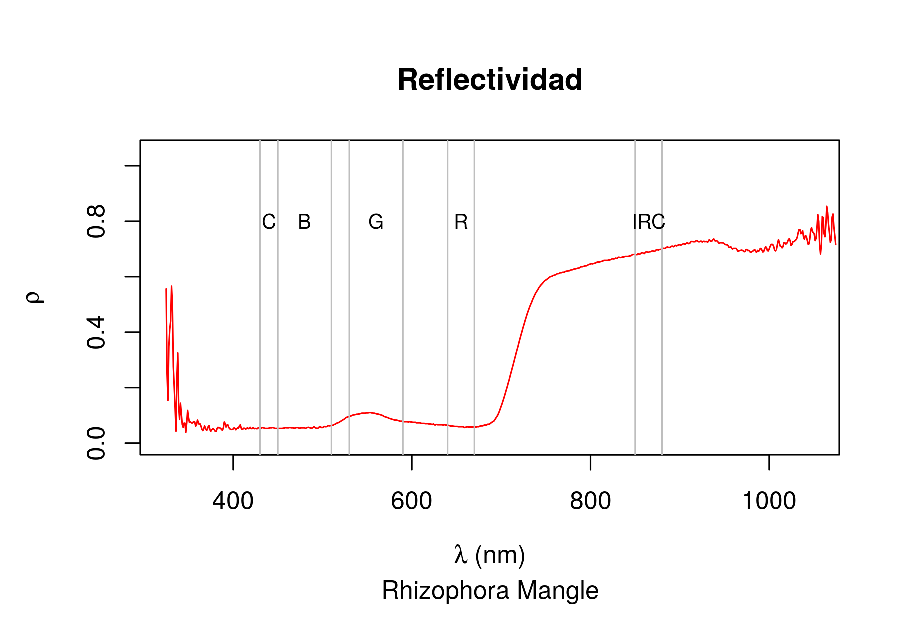
\includegraphics[width=0.8\linewidth]{./Imagenes/RM.eps}
	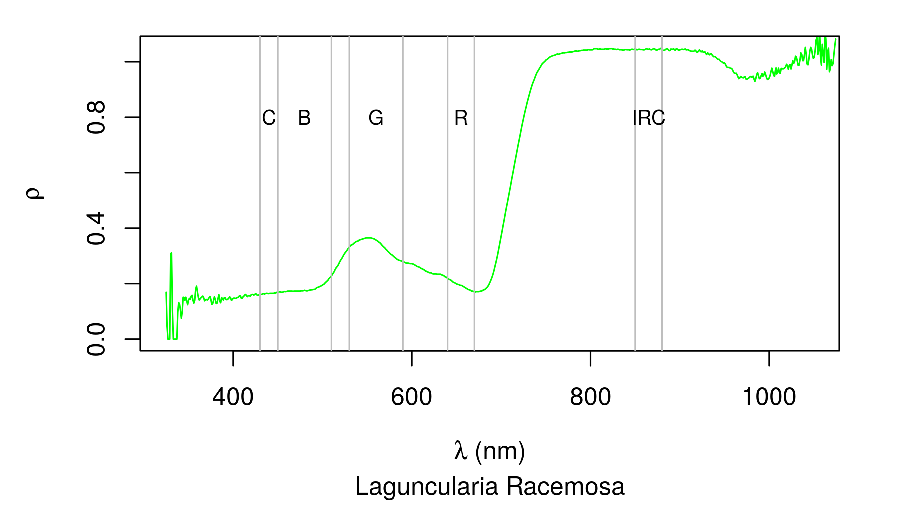
\includegraphics[width=0.8\linewidth]{./Imagenes/LR.eps}
	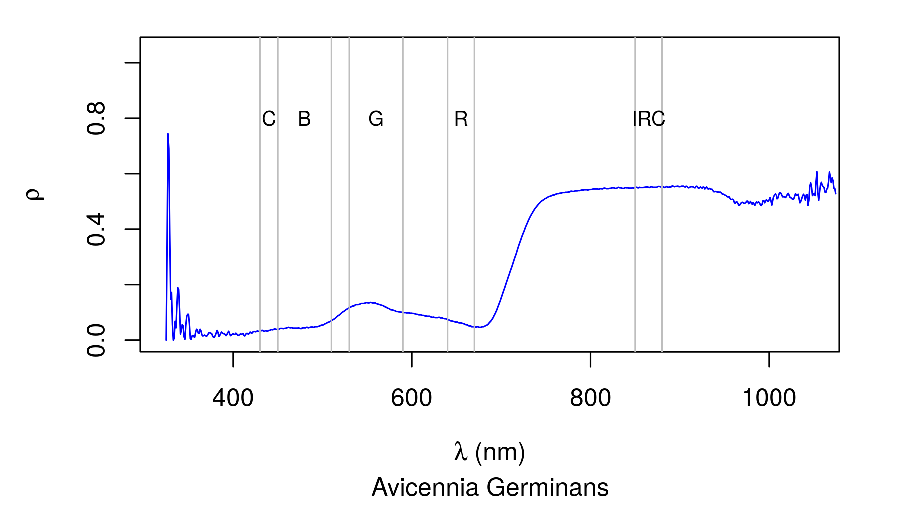
\includegraphics[width=0.8\linewidth]{./Imagenes/AG.eps}
	\captionsetup{font={footnotesize,it}}
	\caption[Firmas espectrales]{Gráficas de las firmas espectrales de las especies de mangle estudiadas. Fuente: Elaboración propia.}
	\label{fig:firmas_espectrales}
\end{figure}

\begin{figure}
	\centering
	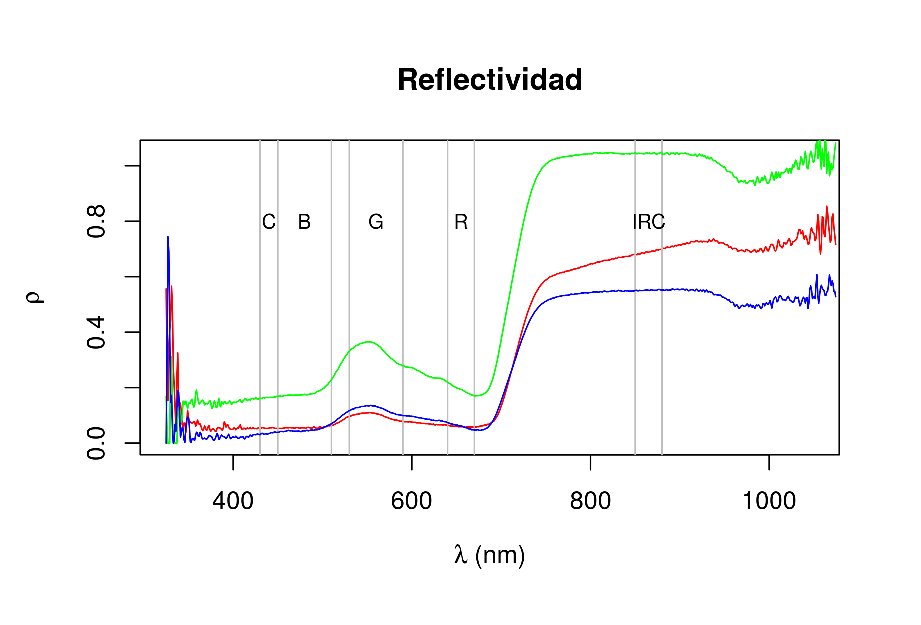
\includegraphics[width=0.8\linewidth]{./Imagenes/ral.eps}
	\captionsetup{font={footnotesize,it}}
	\caption[Firmas espectrales de las tres especies]{Gráfica conjunta de las tres firmas espectrales. Fuente: Elaboración propia.}
	\label{fig:ral}
\end{figure}

Como se aprecia en las figuras los datos presentan unas alteraciones al inicio y al final que son propias del radiómetro. Se procedió a desechar estos datos haciendo un corte de colas entre los valores 420 nm y 900 nm de longitud de onda para preservar lo máximo posible la integridad de los datos y que no afectaran a los análisis de separabilidad. El número de observaciones se reduciría a 481 por las 751 originales. Las gráficas resultantes son las mostradas en las figuras \ref{fig:firmas_espectrales_corte} y \ref{fig:ral_corte}.\Sep

\begin{figure}
	\centering
	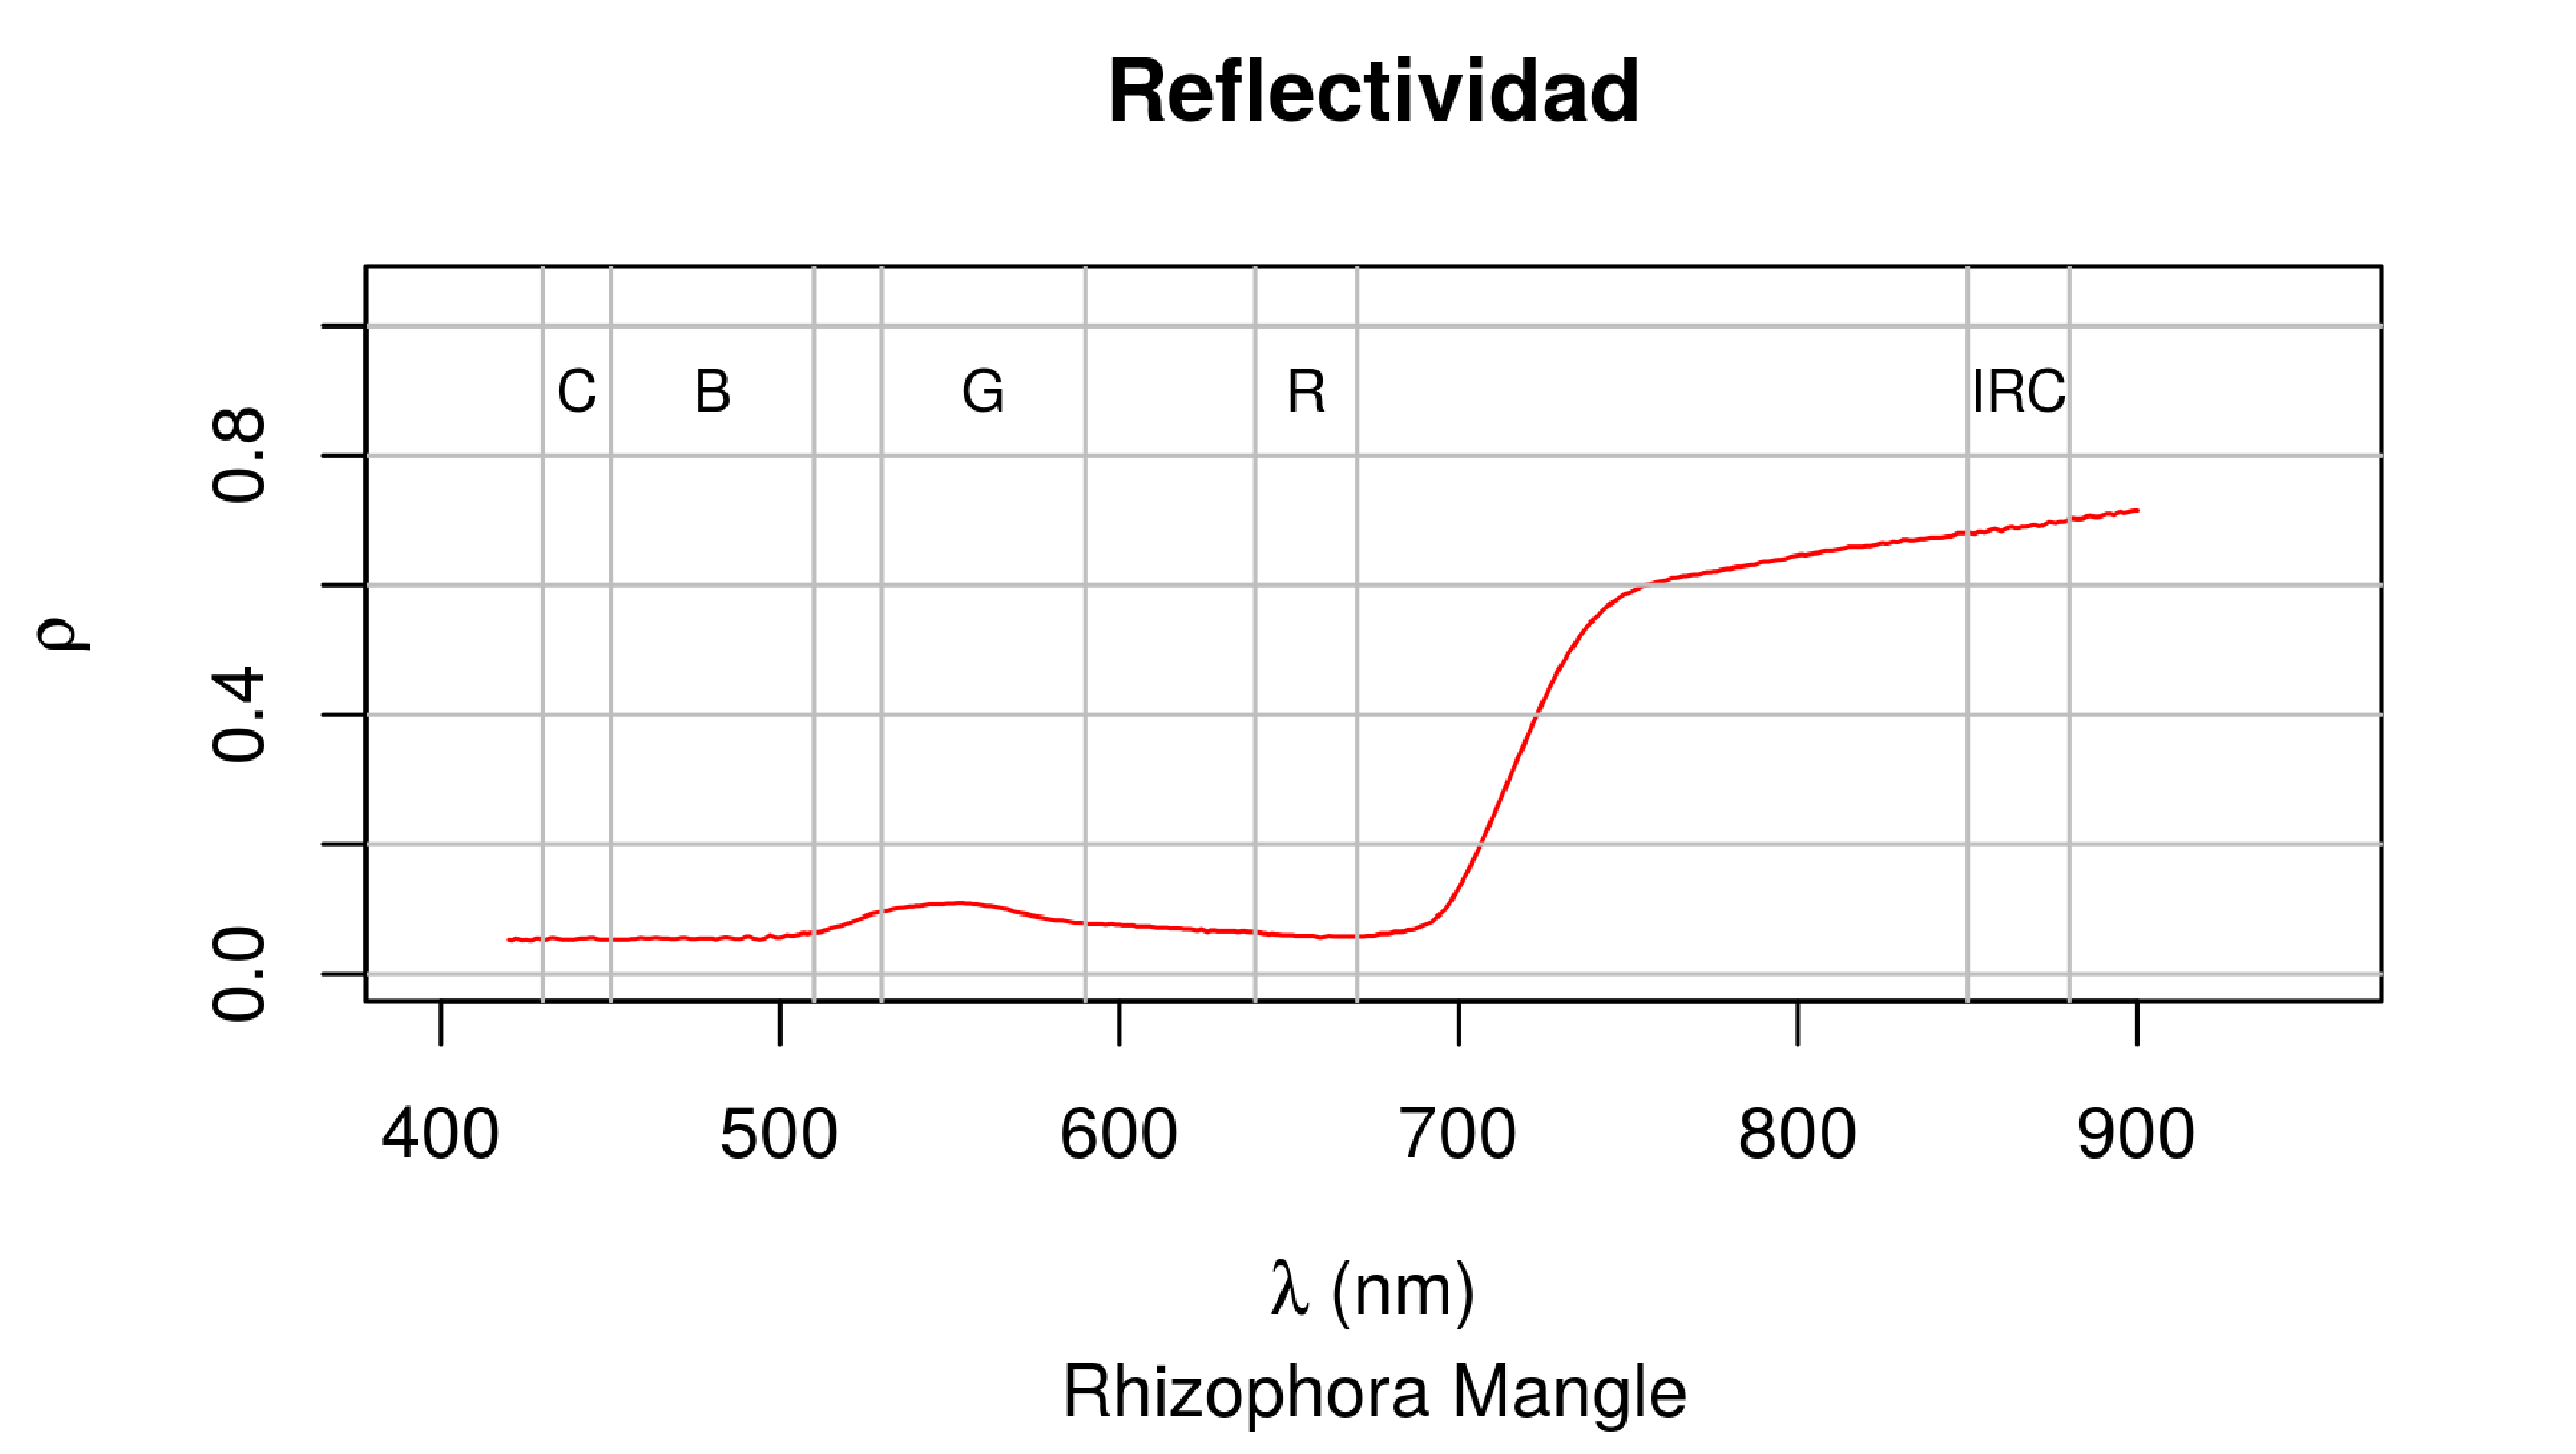
\includegraphics[width=0.8\linewidth]{./Imagenes/RMcorte.eps}
	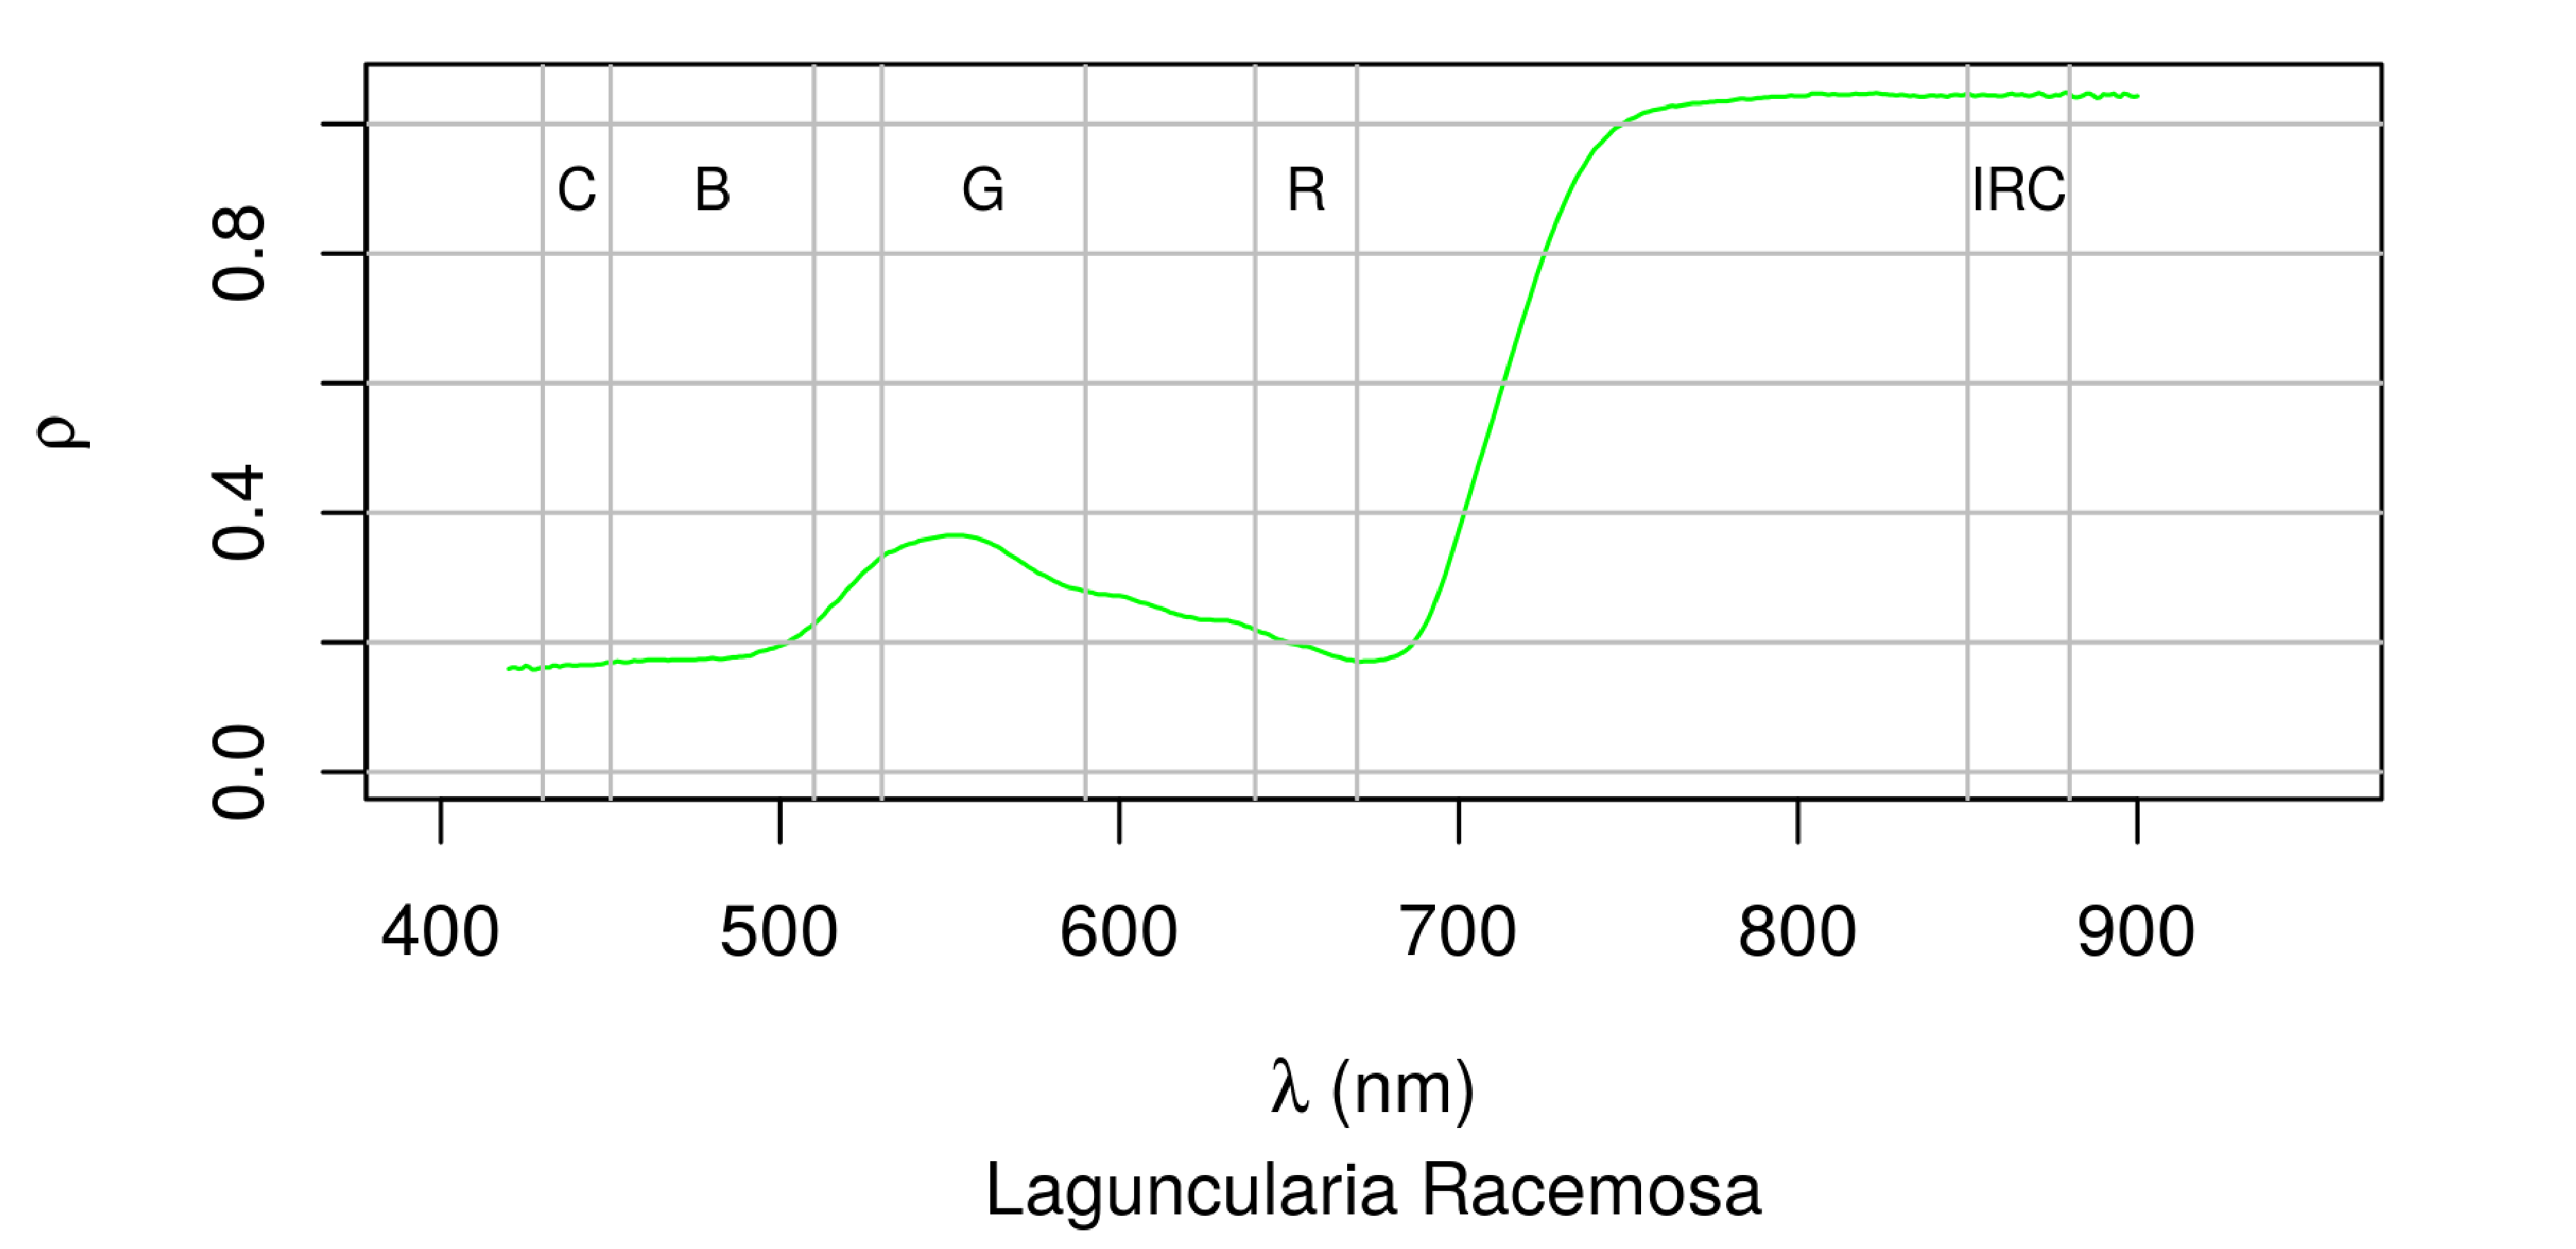
\includegraphics[width=0.8\linewidth]{./Imagenes/LRcorte.eps}
	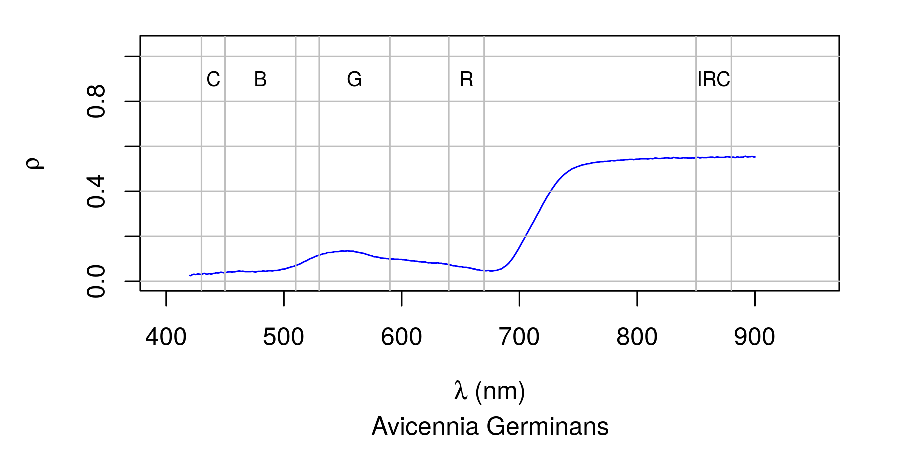
\includegraphics[width=0.8\linewidth]{./Imagenes/AGcorte.eps}
	\captionsetup{font={footnotesize,it}}
	\caption[Firmas espectrales cortadas]{Gráficas de las firmas espectrales de las especies de mangle estudiadas una vez realizado el corte de los datos. Fuente: Elaboración propia.}
	\label{fig:firmas_espectrales_corte}
\end{figure}

\begin{figure}
	\centering
	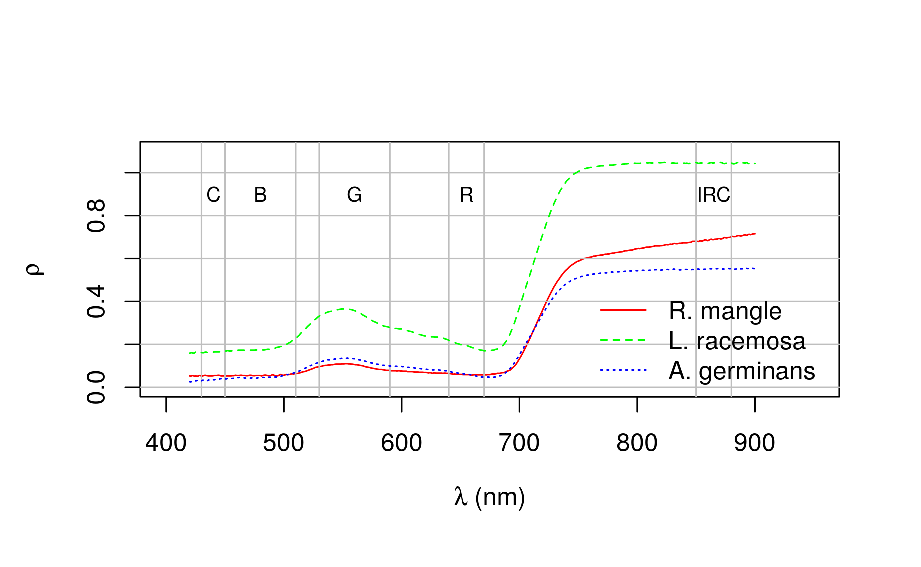
\includegraphics[width=0.8\linewidth]{./Imagenes/ralcorte.eps}
	\captionsetup{font={footnotesize,it}}
	\caption[Firmas espectrales cortadas de las tres especies]{Gráfica conjunta de las tres firmas espectrales una vez realizado el corte de los datos. Fuente: Elaboración propia.}
	\label{fig:ral_corte}
\end{figure}

Las tres especies tienen un máximo local en la banda correspondiente al verde (G), típica de las especies vegetales, así como otro máximo de mayor valor, correspondientes al intervalo de longitud de onda ($\lambda$) en el que está incluida la banda del \ac{IRC}. Este último máximo también es característico de la vegetación e indicaría su grado de salud.\Sep

Por lo tanto el primer vistazo a las gráficas es el esperado, siendo lo más preocupante el aparente parecido entre las especies Rhizophora y Avicennia, que solo se diferencian en el valor del \ac{IRC}.\Sep

En el cuadro siguiente se pueden apreciar los valores medios de cada especie para cada banda de Landsat 8

\begin{table}[ht]
	\centering
	\caption[Valores medios en las bandas Landsat]{Valores medios ara cada banda Landsat. Fuente: Elaboración propia.}
	\begin{tabular}{|c|c|c|c|c|c|}
	\hline
	Especie & Banda 1 (C) & Banda 2 (B) & Banda 3 (G) & Banda 4 (R) & Banda 5 (IRC) \\
	\hline
	\textit{Rhizophora}	& 0.0540 & 0.0561 & 0.0980 & 0.0595 & 0.6895 \\
	\hline	
	\textit{Laguncularia} & 0.1647 & 0.1821 & 0.3345 & 0.1930 & 1.0445 \\
	\hline
	\textit{Avicennia} & 0.0355 & 0.0479 & 0.1218 & 0.0604 & 0.5513 \\
	\hline
	\end{tabular}
\end{table}

\section{Aplicación de los análisis}
\subsection{Índice de Acuerdo Espectral}
Una vez aplicando el script con la función de \ac{IAE} creado en R (figura \ref{fig:IAE}) ya se aprecia que el resultado no es muy bueno, aunque esperado, siendo las diferencias casi inapreciables como se ve en la tabla \ref{tab:Valores_IAE} y en los gráficos de la figura \ref{fig:CB}, donde se aprecia mejor la poca diferencia espectral existente.\Sep

\begin{table}[ht]
	\centering
	\caption[Valores de IAE]{Valores de \ac{IAE} para cada par de especies de mangle. Fuente: Elaboración propia.}
	\begin{tabular}{|c|c|c|c|}
	\hline
	& Rhizophora & Laguncularia & Avicennia \\
	\hline
	Rhizophora & --- & 0.0083 & 0.0062 \\
	\hline
	Laguncularia & 0.0083 & --- & 0.0021 \\
	\hline
	Avicennia & 0.0062 & 0.0021 & --- \\
	\hline
	\end{tabular}
	\label{tab:Valores_IAE}
\end{table}

Las diferencias en este método son bajas debido a que se trata de tres especies que, aunque no sean de la misma familia, si son vegetales y coexisten formando asociación en el mismo ecosistema. De haber estudiado la diferencia entre especie vegetal, suelo y agua por ejemplo, las diferencias habrían sido más notables debido a la diferencia de valor medio de la respuesta espectral. En este caso, el valor medio de las tres especies sería el mostrado en la tabla siguiente:

\begin{table}[ht]
	\centering
	\caption[Valores medios de la respuesta espectral]{Valor medio de la respuesta espectral para cada especie.}
	\begin{tabular}{|c|c|c|}
	\hline
	ESPECIE & $\rho$ MEDIA & CORTE EN $\lambda$ (nm)\\
	\hline
	Rhizophora & 0.2897692 & 714	\\
	\hline
	Laguncularia & 0.5424927 & 710\\
	\hline
	Avicennia & 0.2530166 & 711\\
	\hline
	\end{tabular}
	\label{tab:mediaIAE}
\end{table}

El corte en $\lambda$ que se menciona en el cuadro \ref{tab:mediaIAE} se refiere al valor de longitud de onda a partir del cual la reflectancia es mayor a la media y por tanto se provoca una cambio en el valor binario de 0 a 1 donde, de tener un mayor rango de longitud de onda observada habría más de un cambio. Se observan unos valores similares de $\lambda$ para las tres especies, pero donde sí se notan diferencias son en el valor medio de la reflectancia, siendo el de la Laguncularia notablemente superior al de las otras dos especies.

\begin{figure}
	\centering
	\includegraphics[width=0.8\linewidth]{./Imagenes/IAE_RM.eps}
	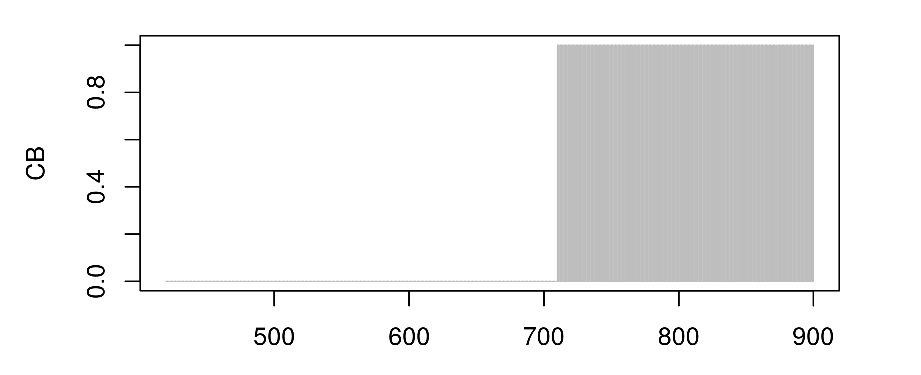
\includegraphics[width=0.8\linewidth]{./Imagenes/IAE_LR.eps}
	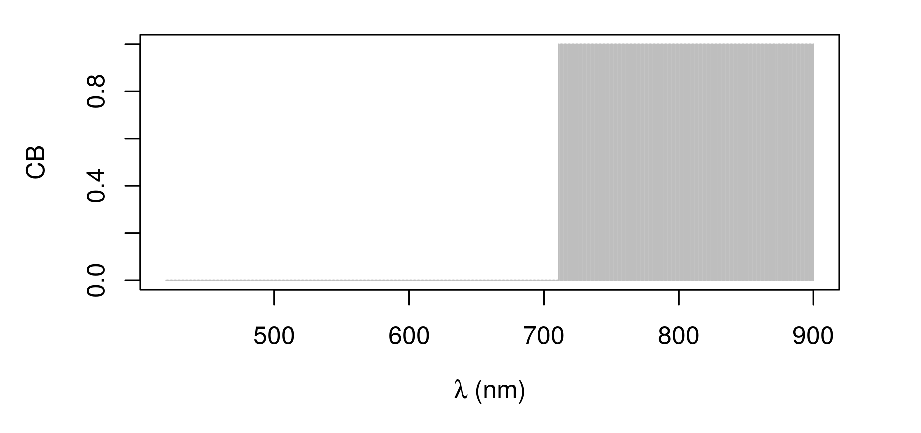
\includegraphics[width=0.8\linewidth]{./Imagenes/IAE_AG.eps}
	\captionsetup{font={footnotesize,it}}
	\caption[Gráficas de combinación binaria]{Gráficas de combinación binaria de las tres especies de mangle, por orden Rhizophora, Laguncularia y Avicennia. Fuente: Elaboración propia.}
	\label{fig:CB}
\end{figure}

\subsection{Continuum Removal}

Para el correcto funcionamiento del análisis se procedió a crear una matriz de 3x481 donde las filas corresponden a las tres especies analizadas y las columnas al valor de longitud de onda. El fin es el de presentar de mejor forma los datos en la función de \ac{CR} de R y aunque el resultado es el mismo, que haciéndolo una por una, nos permite obtener este de forma más rápida y con menos pasos.\Sep

El script de la funcion en R previamente presentado en la figura \ref{fig:CR} sufre cambios, quedando de la siguiente manera:\SmallSep

\begin{figure}[ht]
	\centering
	\begin{lstlisting}[language = R, frame = single]
require(prospectr)
matriz <- matrix(c(RhizophoraCorte$V5,LagunculariaCorte$V5,
                   AvicenniaCorte$V5),
                 byrow=TRUE,
                 nrow=3,
                 ncol=481)
bandas <- mangle1corte$V4
cr <- continuumRemoval(matriz, bandas)
matplot(bandas, t(matriz), type="l", ylim=c(0,1))
matlines(bandas, t(cr2))
	\end{lstlisting}
	\captionsetup{font={footnotesize,it}}
	\caption[Función modificada de CR]{Script modificado de la función de CR escrita en R. Fuente: Elaboración propia.}
	\label{fig:CRmodificado}
\end{figure}	

Donde ``manglencorte'' es el archivo de datos con el corte realizado para cada especie como se explicó anteriormente. Se crea un objeto llamado ``bandas'' tomando los valores de la fila V4 de cualquiera de los archivos de datos. Se crea la gráfica con el comandos ``matplot'' y con ``matlines'' se superpone la gráfica propia del método \ac{CR}. Con el comando inicial ``require(prospectr)'' nos aseguramos que está correctamente cargado el paquete necesario para realizar las operaciones que siguen en el script \citep{stevens2014introduction}. \Sep

En la gráfica de la figura \ref{fig:GraficaCR} se pueden observar las diferencias entre las tres especies que nos indica este tipo de análisis. Son tres los aspectos de esta gráfica a analizar: la profundidad y anchura de las partes convexas y la posición de los puntos mínimos. En gris la gráfica de reflectividad de cada especie.\Sep

\begin{figure}
	\centering
	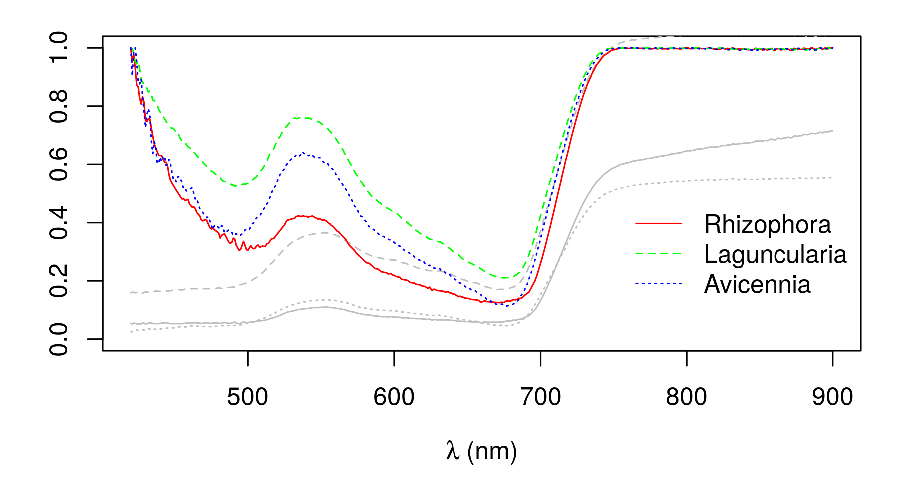
\includegraphics[width=0.8\linewidth]{./Imagenes/ContinuumR2.eps}
	\captionsetup{font={footnotesize,it}}
	\caption[Gráfica de Continuum Removal]{Gráfica de continuum removal para las tres especies de mangle. Fuente: Elaboración propia.}
	\label{fig:GraficaCR}
\end{figure}

En cuanto a la profundidad se observa una clara absorción en torno a los 490 nm y los 680 nm de las tres especies. En el caso de la Avicennia esta absorción es más acusada en ambos puntos. Rhizophora y Laguncularia muestran un comportamiento similar en la primera zona mientras que en la segunda la Laguncularia no muestra la absorción de la Rhizophora.\Sep

En cuanto a la anchura lo más llamativo es la amplitud de los valores de la Rhizophora en torno a los valores centrales de la observación.

\subsection{Clasificación angular}
Una vez aplicado el script de R de la función de clasificación angular (figura \ref{fig:AE}), los valores son los de la siguiente tabla:

\begin{table}[ht]
	\centering
	\caption[Valores de Ángulo Espectral]{Valores del Ángulo Espectral.}
	\begin{tabular}{|c|c|c|c|}
	\hline
	& Rhizophora & Laguncularia & Avicennia \\
	\hline
	Rhizophora & --- & 0.1651 & 0.0752 \\
	\hline
	Laguncularia & 0.1651 & --- & 0.1062 \\
	\hline
	Avicennia & 0.0752 & 0.1062 & --- \\
	\hline
	\end{tabular}
\end{table}

Se puede observar una mayor separabilidad entre Rhizophora y Laguncularia, siendo menor en las otras combinaciones.